% !TEX root = ./proj_report.tex
\graphicspath{{mehul_pics/}}% Set graphics path location

\section{Sharpness Metric}
Often in image sharpening, the sharpness criteria is decided by human visual systems, but this can be a hurdle if the aim is to automate the process with minimum user input and interference. This required the study of robust sharpness metric/s which could compare the performance across different filters in image restoration with or without a reference clear image. There are a variety of metrics that can be used to determine the sharpness of an image, but for the purpose of this analysis we are going to focus on three metrics:

\begin{enumerate}
\item {\bf Gradient Index} \\
The Gradient Index method is based on the very simple idea that as an image gets blurred, the features are diminished and tend towards a constant value. This is quantified by numerically computing the gradients and averaging them to provide a single value. As the image gets blurrier, the index will decrease. 

Due to its simplicity, this method is not very effective when noise is present. Noise introduces high gradients into the image, and consequentially biases the result towards a much higher value than the one expected based on its sharpness quality.  

The based code that was further modified for this project was obtained from the MATLAB exchange and was created by Tolga Birdal.

\item {\bf Structural Similarity Index (SSI)~\cite{Wang:2004}} \\
The Structural Similarity Method uses a change in luminosity of the blurred image, and compares it to a reference clear image. The closer this index is to a value of one, the shaper the image is. Unfortunately, this metric is not useful for real images, since it requires a clear image as a reference for the metric.

\item {\bf Just Noticeable Blur (JNB)~\cite{Ferzli:2009}} \\
The Just Noticeable Blur method uses the idea that as an image gets blurry, the width of the edges start to increase and blend with the background. By specifying an empirically obtained threshold, it can quantify at which level of blurriness the average human eye starts to perceive blur. The higher the index, the blurrier the image is expected to be.
\end{enumerate}

\subsection{Train Image: Informational Sign}
To validate the implementation and better understand the functionality of the sharpness metrics, the image of an informational sign was taken and blurred. The results at three levels of blur are show in Figure~\ref{fig:train_metrics}.

\begin{figure}[h!]
        \centering
        \begin{subfigure}[b]{0.35\textwidth}
                \centering
                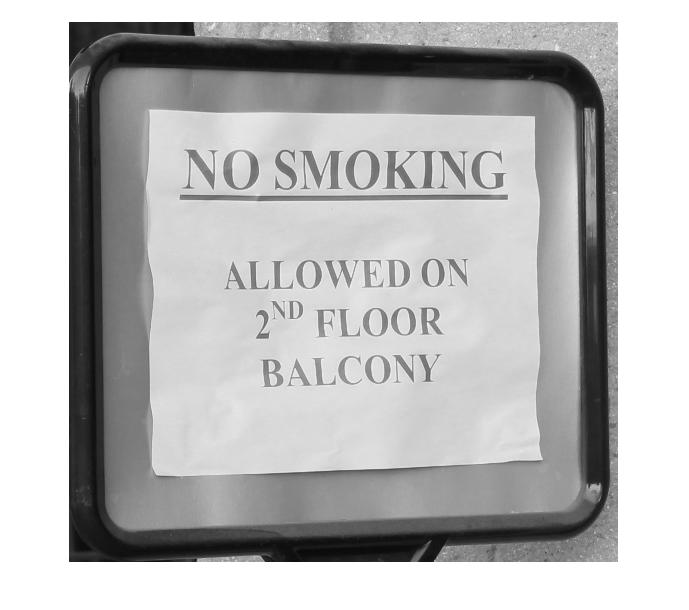
\includegraphics[width=\textwidth]{true.jpg}
                \caption{Sharp Image..\newline $Grad=0.0183$ ; $SSI=1.000$ ;\newline $JNB=8.4419$}
               
        \end{subfigure}
        \hspace{.6cm}
        \begin{subfigure}[b]{0.35\textwidth}
                 \centering
                 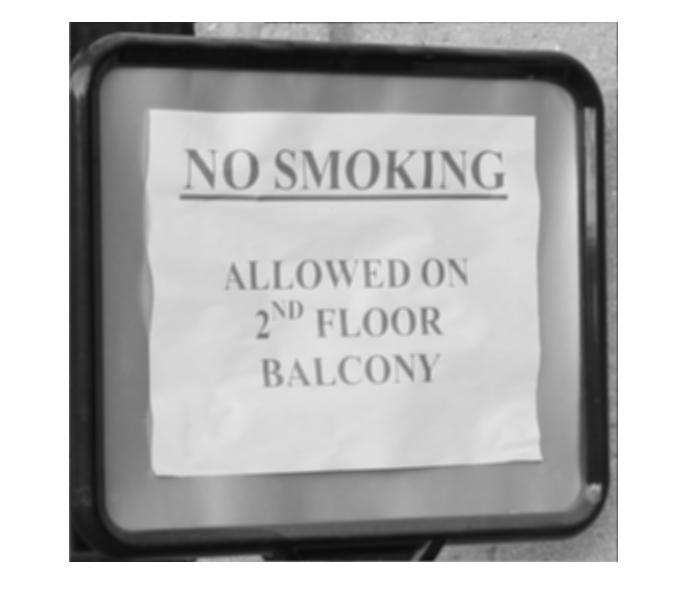
\includegraphics[width=\textwidth]{sign_D.jpg}
                 \caption{Image blurred by a disk.\newline $Grad=0.0145$ ; $SSI=1.000$ ;\newline $JNB=5.6732$}
                       
        \end{subfigure}
        \hspace{.6cm}
        \begin{subfigure}[b]{0.35\textwidth}
                \centering
                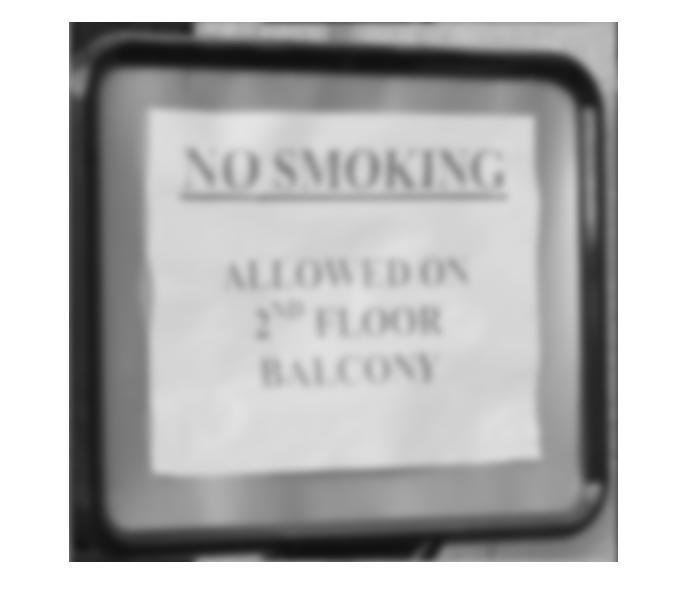
\includegraphics[width=\textwidth]{sign_G.jpg}
                \caption{Image blurred by a Gaussian.\newline $Grad=0.0108$ ; $SSI=0.9998$ ;\newline $JNB=2.8083$} 
        \end{subfigure} 
       
        \caption{As the blur increases in the image, the gradient value decreases, the SSI decreases and the JNB increases. The responses are independent of the blur type, and since its understood the noise levels will bias the values for some of the  coefficients, it has been ignored for this validation study.} \label{fig:train_metrics}
\end{figure}

\noindent From the study shown in Figure~\ref{fig:train_metrics}, the least reliable metric to determine sharpness is SSI in additon to require a reference image, therefore this will not be considered for the analysis of real images.

\subsection{Real Image: Friends}
Having studied different filters and sharpness metrics, a rudimentary algorithm was implemented to sharpen images with minimum user input. As the state the code is currently in, it requires an initial PSF guess from the user, and iterates through different filters and different PSF sizes with the flexibility of using multiple PSFs together, plotting the sharpness metrics, and asking for user input once in a while to know whether the program should continue looking for the solution or stop if the user is satisfied with the sharpness level. This code was designed as a preprocessing tool for image data analysis. Often times the type of image noise and blur present is consistent with the set of images procured from a common image capturing mechanism. By determining the optimum filter, PSF shape/s, and size that best sharpen an image, this code will help determine the optimum filter and characteristics for the complete data set. Figure~\ref{fig:friends} is an example of the analysis done in a real blurry image.

\begin{figure}[H]
        \centering
        \begin{subfigure}[b]{0.49\textwidth}
                \centering
                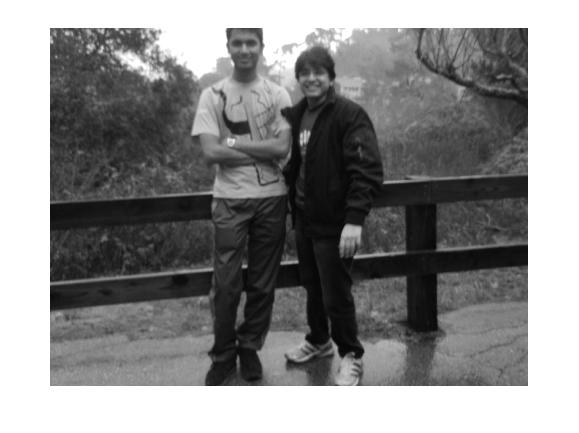
\includegraphics[width=\textwidth]{blur_personal.jpg}
                \caption{Blurry no reference image.}
        \end{subfigure}
        \begin{subfigure}[b]{0.49\textwidth}
                 \centering
                 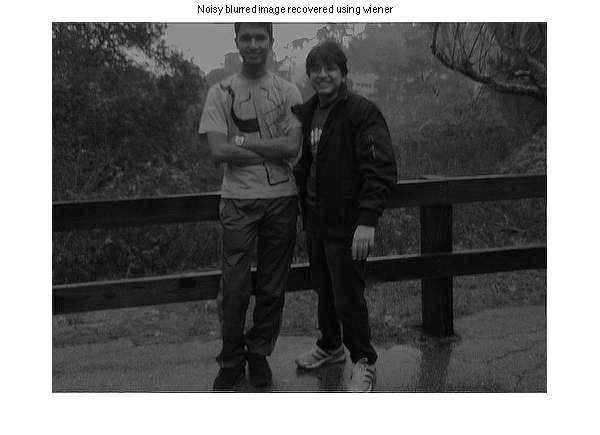
\includegraphics[width=\textwidth]{sharp_personal_bright.jpg}
                 \caption{Image sharpened by the Wiener filter.}
                 \label{fig:friends}
                       
        \end{subfigure}
              
        \caption{No reference Image sharpened using sharpness metrics and automated iterative sharpening code. The initial guess for the underlying PSF was a disk with radius 8 pixels. Sharpening was stopped when the plotted metrics showed an increase in criteria indicating optimum PSF shape and size had been reached. The filter that worked best is Wiener filter and the final image was enhanced using the underlying PSF to be a combination of disk and Gaussian. Luminance in the restored image is affected by the high magnitude of noise in the original image.} \label{fig:true_metrics}
\end{figure}

\newpage